\documentclass[11pt,a4paper]{article}
\usepackage[margin=2.2cm]{geometry}
\usepackage{amsmath,amssymb,bm}
\usepackage{graphicx,float,booktabs,caption,subcaption}
\usepackage{xcolor}
\usepackage{listings}
\usepackage{tikz}
\usetikzlibrary{shapes.geometric,arrows.meta,positioning,calc}
\usepackage[colorlinks=true,linkcolor=blue!50!black,urlcolor=blue!50!black,citecolor=blue!50!black]{hyperref}
\usepackage{fancyhdr}
\pagestyle{fancy}\fancyhf{}\lhead{\small Karthick J (OE23S018), IIT Madras}\rhead{\small\leftmark}\cfoot{\thepage}
\definecolor{codebg}{rgb}{0.97,0.97,0.97}
\lstset{basicstyle=\ttfamily\scriptsize,backgroundcolor=\color{codebg},frame=single,breaklines=true,
 keywordstyle=\color{blue!60!black}\bfseries,commentstyle=\color{green!40!black},stringstyle=\color{red!50!black},
 numbers=left,numberstyle=\tiny\color{gray},showstringspaces=false,tabsize=4,columns=fullflexible,
 literate={²}{{$^2$}}1 {³}{{$^3$}}1 {°}{{$^\circ$}}1 {Δ}{{$\Delta$}}1 {ρ}{{$\rho$}}1 {μ}{{$\mu$}}1 {ω}{{$\omega$}}1 {ψ}{{$\psi$}}1 {α}{{$\alpha$}}1 {ν}{{$\nu$}}1 {τ}{{$\tau$}}1 {–}{{-}}1 {—}{{-}}1 {’}{{'}}1 {“}{{"}}1 {”}{{"}}1 {→}{{$\to$}}1 {≤}{{$\le$}}1 {≥}{{$\ge$}}1 {×}{{$\times$}}1 {±}{{$\pm$}}1 {·}{{$\cdot$}}1 {∂}{{$\partial$}}1 {∇}{{$\nabla$}}1 {γ}{{$\gamma$}}1 {ε}{{$\varepsilon$}}1 {μ}{{$\mu$}}1 {├}{{+}}1 {─}{{-}}1 {│}{{|}}1 {▶}{{>}}1 {▼}{{v}}1 {┌}{{+}}1 {┐}{{+}}1 {└}{{+}}1 {┘}{{+}}1 {┬}{{+}}1 {┴}{{+}}1}
\tikzset{
 startstop/.style={rectangle,rounded corners=6pt,minimum width=3.2cm,minimum height=0.8cm,text centered,draw=black,fill=red!12,font=\small},
 process/.style={rectangle,minimum width=4.6cm,minimum height=0.8cm,text centered,text width=5.6cm,draw=black,fill=blue!8,font=\small},
 decision/.style={diamond,aspect=2.6,text centered,text width=3.2cm,draw=black,fill=green!12,font=\small,inner sep=1pt},
 io/.style={trapezium,trapezium left angle=72,trapezium right angle=108,minimum width=3.6cm,minimum height=0.8cm,text centered,text width=4.6cm,draw=black,fill=orange!15,font=\small},
 arrow/.style={thick,-{Stealth[length=2.5mm]}}}
\setlength{\parskip}{4pt}\setlength{\parindent}{0pt}

\title{\textbf{Lid-Driven Cavity Flow at $\mathrm{Re}=100$}\\[2pt]\large Incompressible Navier--Stokes Solution with the SMAC Projection Method on a Staggered Grid (C)\\[2pt]\normalsize Course Project 5 -- AM5630 Foundation of Computational Fluid Dynamics (Computer Assignment 3, Jan--May 2024)}
\author{Karthick J (OE23S018)\\Department of Ocean Engineering, IIT Madras}
\date{Revised report, October 2026}
\begin{document}\maketitle
\begin{abstract}
Steady two-dimensional incompressible flow in a unit square cavity driven by a sliding lid is computed at $\mathrm{Re}=100$ with the Simplified Marker-And-Cell (SMAC) fractional-step method on a staggered (MAC) grid of $99\times99$ cells. The original assignment code fixed the program structure (constants, \texttt{compute\_pressure}, \texttt{update\_velocity}, \texttt{compute\_vorticity}, time loop and output files) but did not solve the governing equations and terminated with a segmentation fault; the function bodies were completed here following the SMAC algorithm stated in the original report. Time marching ($\Delta t=10^{-3}$, CFL $=0.099$) reaches steady state ($\max|u^{n+1}-u^n|<10^{-7}$) at $t=13.56$. The primary-vortex stream function $\psi_{min}=-0.10337$ and centre $(0.616,0.737)$ agree with the benchmark of Ghia, Ghia \& Shin (1982) [$-0.10342$ at $(0.617,0.734)$] to within $0.05\%$ and one cell, the centreline velocities agree to within $\max|\Delta u|=0.005$ and $\max|\Delta v|=0.009$, and both secondary corner eddies are resolved and converge towards the benchmark strengths under grid refinement.
\end{abstract}
\tableofcontents\newpage

\section{Problem definition}
A unit square cavity is filled with an incompressible Newtonian fluid. The top wall (lid) slides at $U=1$; the other three walls are at rest. With $L$ and $U$ as scales, the non-dimensional equations are
\begin{align}
\nabla\cdot\mathbf{u}&=0, \label{eq:cont}\\
\frac{\partial\mathbf{u}}{\partial t}+\nabla\cdot(\mathbf{u}\mathbf{u})&=-\nabla p+\frac{1}{\mathrm{Re}}\nabla^2\mathbf{u},\qquad \mathrm{Re}=\frac{UL}{\nu}=100, \label{eq:mom}
\end{align}
with $\mathbf{u}=(u,v)$, no slip on all walls, $u=1$, $v=0$ on the lid, and $\mathbf{u}=0$ at $t=0$. Pressure needs no physical boundary condition; the projection step imposes $\partial\phi/\partial n=0$ on the pressure correction, which is consistent with $\mathbf{u}\cdot\mathbf{n}=0$. The steady state is obtained as the long-time limit of the transient problem.

\section{Numerical method}
\subsection{Staggered (MAC) grid}
\begin{figure}[H]\centering
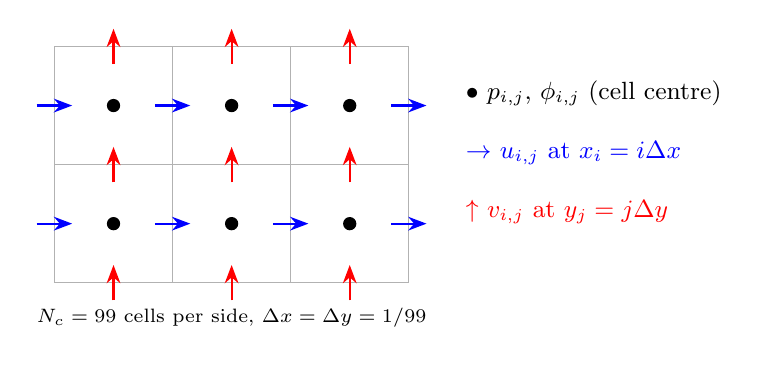
\begin{tikzpicture}[scale=1.5]
\draw[gray!60](0,0)grid(3,2);
\foreach \i in {0,1,2}\foreach \j in {0,1}{\fill(\i+0.5,\j+0.5)circle(1.6pt);}
\foreach \i in {0,1,2,3}\foreach \j in {0,1}{\draw[-{Stealth},blue,thick](\i-0.15,\j+0.5)--(\i+0.15,\j+0.5);}
\foreach \i in {0,1,2}\foreach \j in {0,1,2}{\draw[-{Stealth},red,thick](\i+0.5,\j-0.15)--(\i+0.5,\j+0.15);}
\node[right,font=\small] at (3.4,1.6){$\bullet$ $p_{i,j}$, $\phi_{i,j}$ (cell centre)};
\node[right,font=\small,blue] at (3.4,1.1){$\rightarrow$ $u_{i,j}$ at $x_i=i\Delta x$};
\node[right,font=\small,red] at (3.4,0.6){$\uparrow$ $v_{i,j}$ at $y_j=j\Delta y$};
\node[font=\scriptsize] at (1.5,-0.3){$N_c=99$ cells per side, $\Delta x=\Delta y=1/99$};
\end{tikzpicture}
\caption{MAC arrangement. Velocities on faces and pressure at centres couple pressure and velocity on adjacent points, which prevents the odd--even (checkerboard) pressure decoupling of a collocated central scheme.}\end{figure}
Wall velocities normal to a wall lie on the wall and are set directly ($u=0$ on $x=0,1$; $v=0$ on $y=0,1$). Tangential velocities are imposed through a ghost layer by linear extrapolation:
\begin{equation}u_{i,0}=-u_{i,1},\qquad u_{i,N_c+1}=2U-u_{i,N_c},\qquad v_{0,j}=-v_{1,j},\qquad v_{N_c+1,j}=-v_{N_c,j}.\end{equation}

\subsection{SMAC fractional step}
Each time step $t^n\to t^{n+1}$ consists of:
\begin{enumerate}
\item \textbf{Predictor} with the old pressure (explicit Euler; convective terms in conservative form, second-order central averages to the faces; five-point viscous Laplacian):
\begin{equation}\mathbf{u}^*=\mathbf{u}^n+\Delta t\Big[-\nabla\cdot(\mathbf{u}\mathbf{u})^n+\frac{1}{\mathrm{Re}}\nabla^2\mathbf{u}^n-\nabla p^n\Big].\end{equation}
For example, at the $u$-face $(i,j)$:
$\big[\partial(u^2)/\partial x\big]_{ij}=(\bar u_e^2-\bar u_w^2)/\Delta x$, $\big[\partial(uv)/\partial y\big]_{ij}=(\bar u_n\bar v_n-\bar u_s\bar v_s)/\Delta y$, with bars denoting two-point averages.
\item \textbf{Pressure correction}: requiring $\nabla\cdot\mathbf{u}^{n+1}=0$ for $\mathbf{u}^{n+1}=\mathbf{u}^*-\Delta t\nabla\phi$ gives the Poisson equation
\begin{equation}\nabla^2\phi=\frac{1}{\Delta t}\nabla\cdot\mathbf{u}^*,\qquad \frac{\partial\phi}{\partial n}\Big|_{wall}=0, \label{eq:pp}\end{equation}
discretised with the compact five-point operator (wall links removed for the Neumann condition) and solved by SOR ($\omega=1.85$) to $\max|\delta\phi|<10^{-8}$. The Neumann problem is solvable because $\oint\mathbf{u}^*\cdot\mathbf{n}=0$ (discrete compatibility); $\phi$ is fixed up to a constant, which SOR selects through the zero initial guess.
\item \textbf{Corrector}: $\mathbf{u}^{n+1}=\mathbf{u}^*-\Delta t\nabla\phi$, \;$p^{n+1}=p^n+\phi$.
\end{enumerate}
SMAC differs from the original MAC method in solving for the pressure \emph{increment} $\phi$ rather than for $p$ itself; at steady state $\phi\to0$ and $\mathbf{u}^*\to\mathbf{u}^{n+1}$, so the converged solution satisfies the discrete continuity and momentum equations exactly (to the Poisson tolerance).

\subsection{Stability and accuracy}
The explicit predictor is limited by the convective (CFL) and viscous (diffusion number) conditions and by the cell Reynolds number of central differencing:
\begin{equation}
\mathrm{CFL}=\frac{U\Delta t}{\Delta x}=0.099<1,\qquad d=\frac{\Delta t}{\mathrm{Re}\,\Delta x^2}=0.098<\tfrac14,\qquad \mathrm{Re}_\Delta=\mathrm{Re}\,U\Delta x=1.01\lesssim2 .
\end{equation}
The spatial discretisation is second-order; the time discretisation is first-order but irrelevant for the steady solution.

\subsection{Algorithm and flowchart}
\begin{figure}[H]\centering
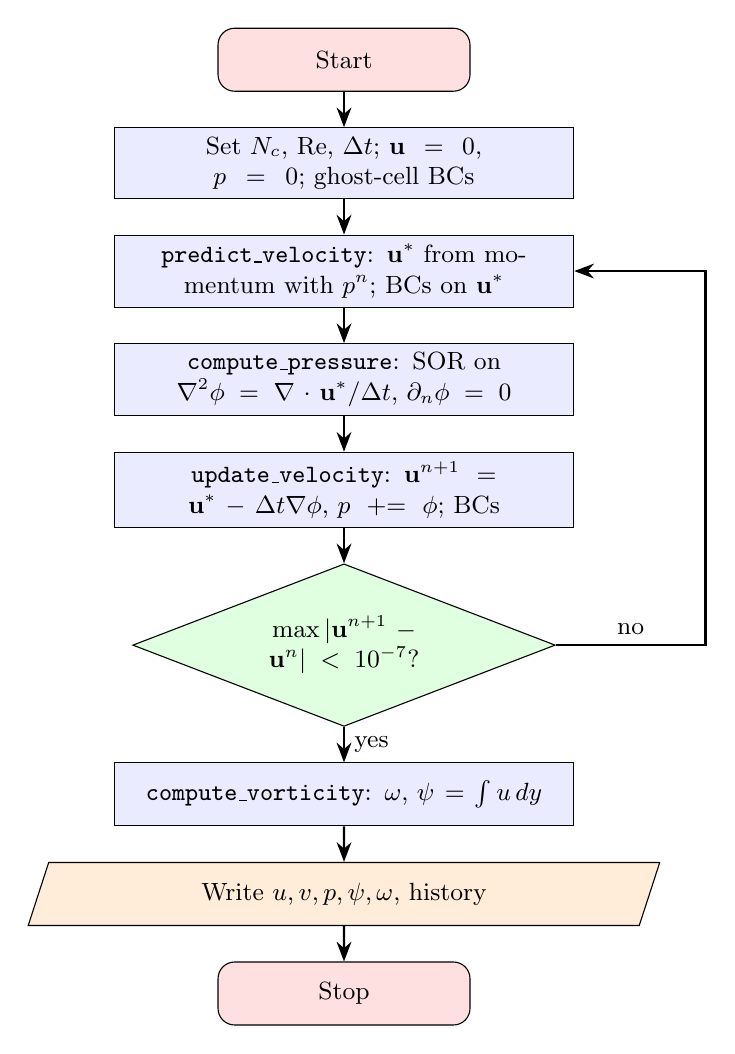
\begin{tikzpicture}[node distance=0.45cm]
\node(s)[startstop]{Start};
\node(i)[process,below=of s]{Set $N_c$, Re, $\Delta t$; $\mathbf{u}=0$, $p=0$; ghost-cell BCs};
\node(pr)[process,below=of i]{\texttt{predict\_velocity}: $\mathbf{u}^*$ from momentum with $p^n$; BCs on $\mathbf{u}^*$};
\node(pp)[process,below=of pr]{\texttt{compute\_pressure}: SOR on $\nabla^2\phi=\nabla\cdot\mathbf{u}^*/\Delta t$, $\partial_n\phi=0$};
\node(co)[process,below=of pp]{\texttt{update\_velocity}: $\mathbf{u}^{n+1}=\mathbf{u}^*-\Delta t\nabla\phi$, $p\mathrel{+}=\phi$; BCs};
\node(d)[decision,below=of co]{$\max|\mathbf{u}^{n+1}-\mathbf{u}^n|<10^{-7}$?};
\node(v)[process,below=of d]{\texttt{compute\_vorticity}: $\omega$, $\psi=\int u\,dy$};
\node(w)[io,below=of v]{Write $u,v,p,\psi,\omega$, history};
\node(e)[startstop,below=of w]{Stop};
\draw[arrow](s)--(i);\draw[arrow](i)--(pr);\draw[arrow](pr)--(pp);\draw[arrow](pp)--(co);\draw[arrow](co)--(d);
\draw[arrow](d)--node[right,font=\small]{yes}(v);\draw[arrow](v)--(w);\draw[arrow](w)--(e);
\draw[arrow](d.east)--node[above,font=\small]{no}++(1.9,0)|-(pr.east);
\end{tikzpicture}\caption{SMAC time-marching loop (\texttt{code/smac\_cavity.c}).}\end{figure}

\section{Code review of the original submission}
The original program (kept in \texttt{original/Assignment\_3\_original.c}) compiles with warnings and terminates with a \textbf{segmentation fault} (exit code 139) before writing any data; all five output files are empty. This is consistent with the original report, which states that the results could not be plotted. The defects were:
\begin{table}[H]\centering\small
\begin{tabular}{p{3.2cm}p{11.9cm}}\toprule
Location & Defect\\\midrule
\texttt{main}: \texttt{double S[i][j], Vor[i][j];} & Variable-length arrays sized by the \emph{uninitialised} loop counters $i,j$ (undefined behaviour): the cause of the crash.\\
\texttt{compute\_pressure} & Not a pressure equation: $p$ is updated with an ad-hoc combination of derivatives of $u$ only ($h_x^2+h_y^2-h_{xx}-h_{yy}-h_{xy}$); $v$ and the velocity divergence do not appear, so continuity is never enforced.\\
\texttt{update\_velocity} & Only the pressure-gradient term is applied: no convection, no viscous term, i.e.\ no momentum equation. The results go to \texttt{unew}, \texttt{vnew}, which are never copied back, so $u$ and $v$ stay zero for all time.\\
boundary conditions & The wall/lid branches sit inside loops that run only over interior indices ($1\ldots N-2$), so they never execute: the lid velocity is never imposed and nothing drives the flow.\\
\texttt{compute\_vorticity} & Empty loop body.\\
\#define \texttt{DX 1.0 / (NX - 1)} & Missing brackets: \texttt{a / DX} expands to \texttt{a / 1.0 / (NX-1)}.\\
\texttt{NT 1000} & $t_{end}=1$: far from steady state ($\approx13.6$ needed).\\
\texttt{float} & Single precision prevents converging the Poisson equation to small tolerances.\\\bottomrule
\end{tabular}\caption{Defects in the original code.}\end{table}
\textbf{What was done.} In this revision the program structure, constants (Re $=100$, $\Delta t=10^{-3}$, 100 grid lines per side), function names, time loop and output files were kept, and the function bodies were completed to implement the algorithm of Section~2. Additions are marked \texttt{[COMPLETED]}, \texttt{[FIX]} or \texttt{[ADDED]} in \texttt{code/smac\_cavity.c}. Because the numerical core was written during this revision, the solver should be regarded as a completed version of the assignment rather than the original submission.

\section{Results}
\subsection{Convergence to steady state}
\begin{figure}[H]\centering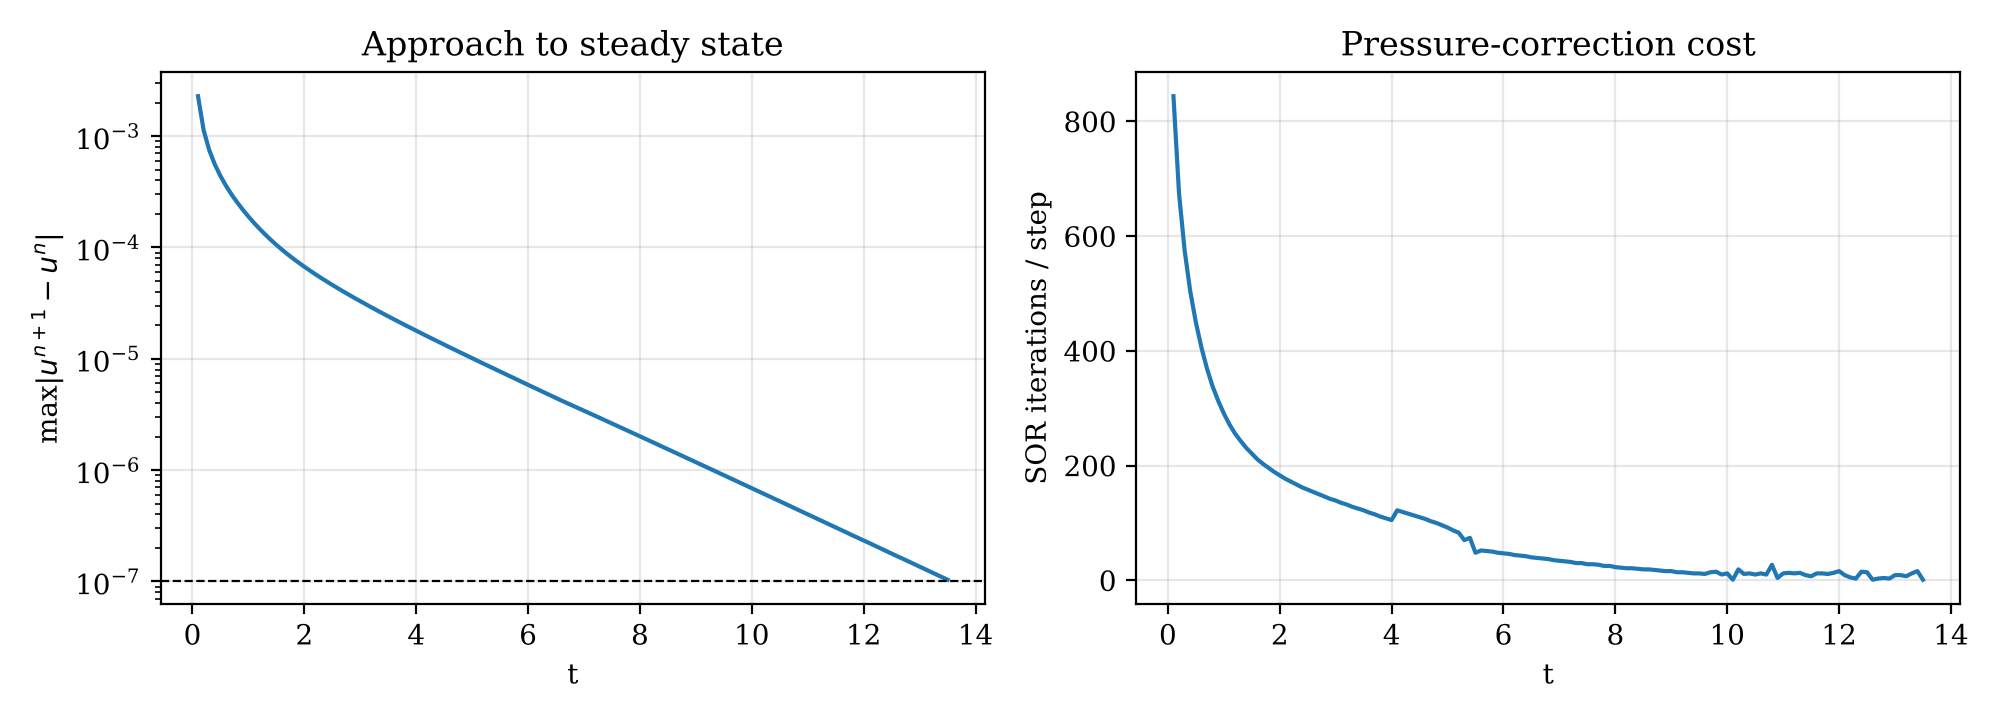
\includegraphics[width=\textwidth]{../results/fig3_convergence_history.png}
\caption{Maximum velocity change per step and SOR iterations per step for the $99\times99$ run.}\end{figure}
The velocity change decays exponentially, at a rate set by the slowest viscous mode, and falls below $10^{-7}$ at step 13\,563 ($t=13.56$). The number of SOR sweeps per step drops from several hundred at start-up to about 10 as $\phi\to0$, the expected behaviour of an incremental-pressure (SMAC) formulation. The run takes about 3.5 minutes on one CPU core.

\subsection{Flow structure}
\begin{figure}[H]\centering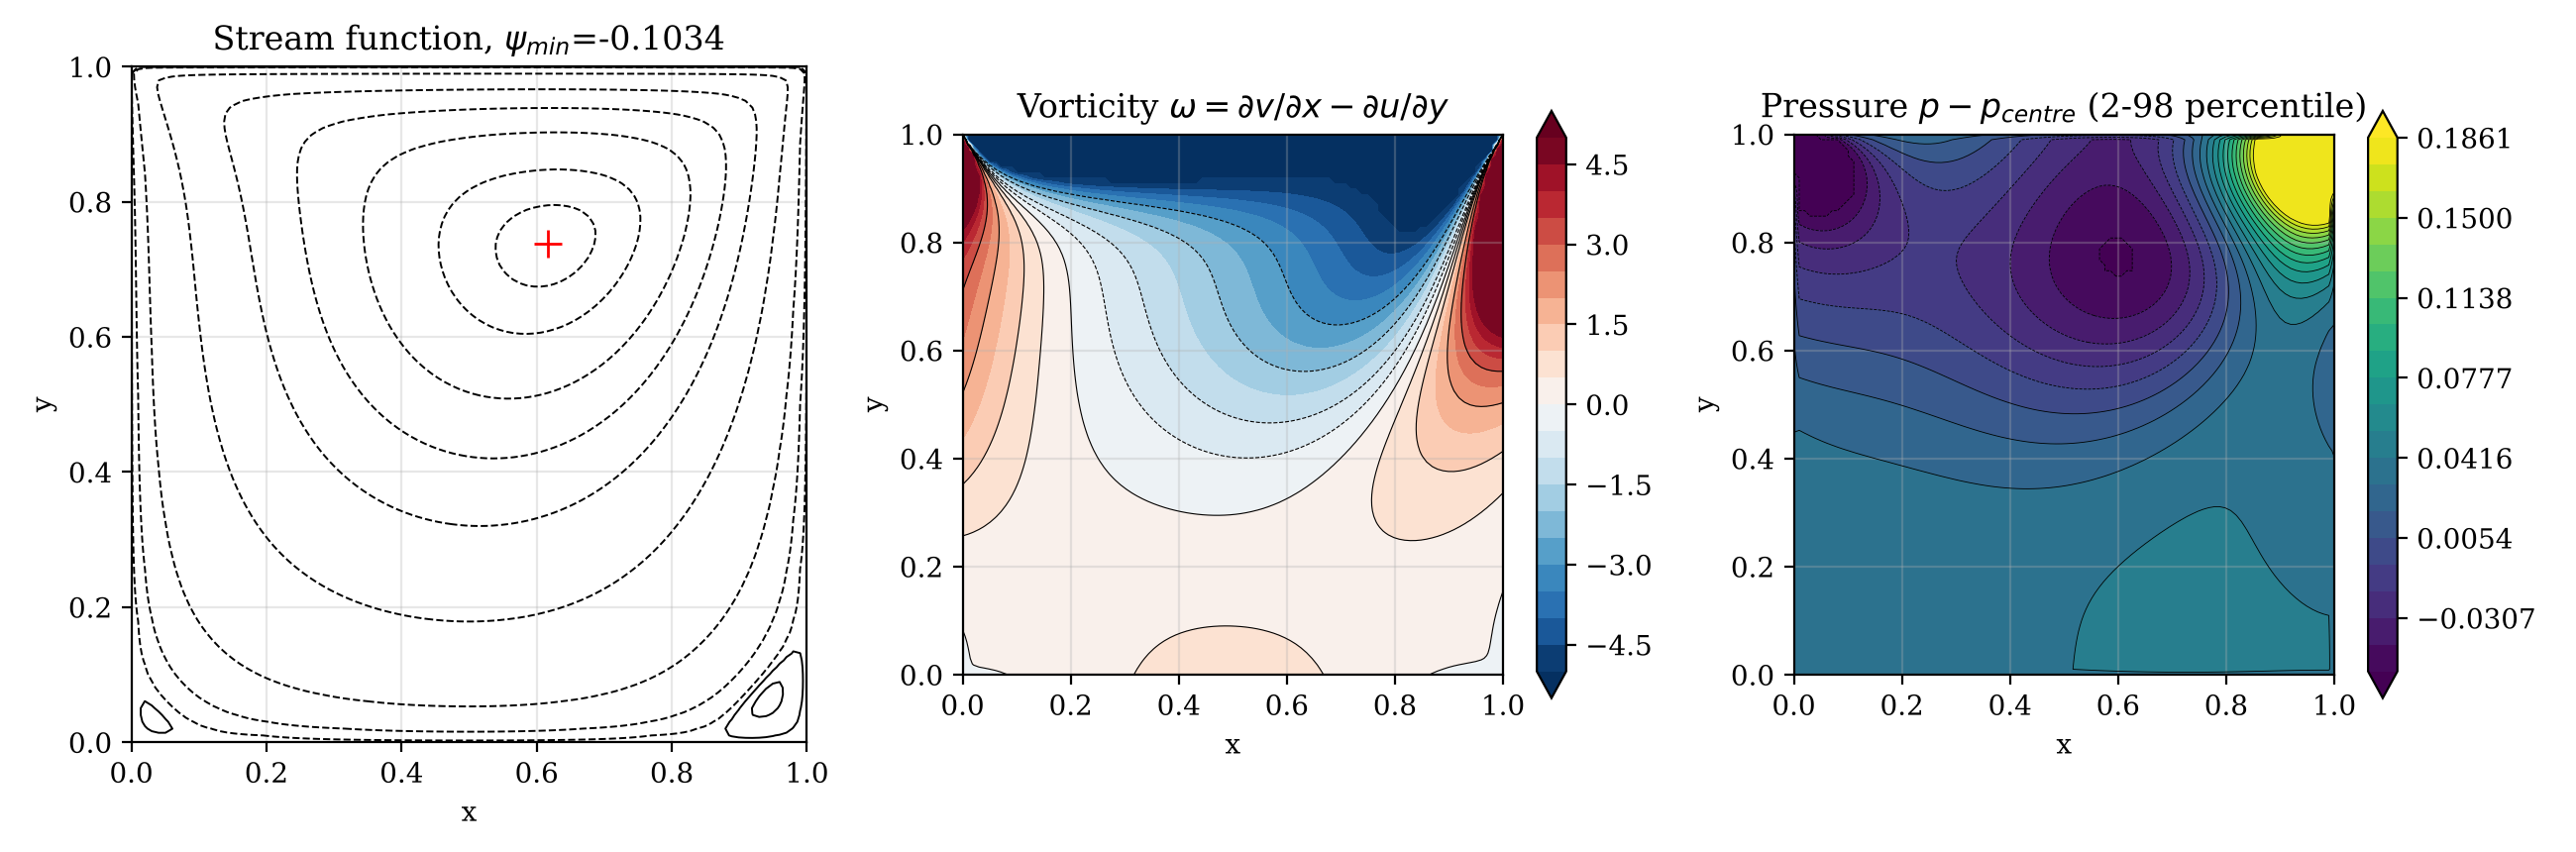
\includegraphics[width=\textwidth]{../results/fig1_streamlines_vorticity_pressure.png}
\caption{Stream function (primary vortex centre marked), vorticity and pressure for the $99\times99$ grid.}\end{figure}
\begin{figure}[H]\centering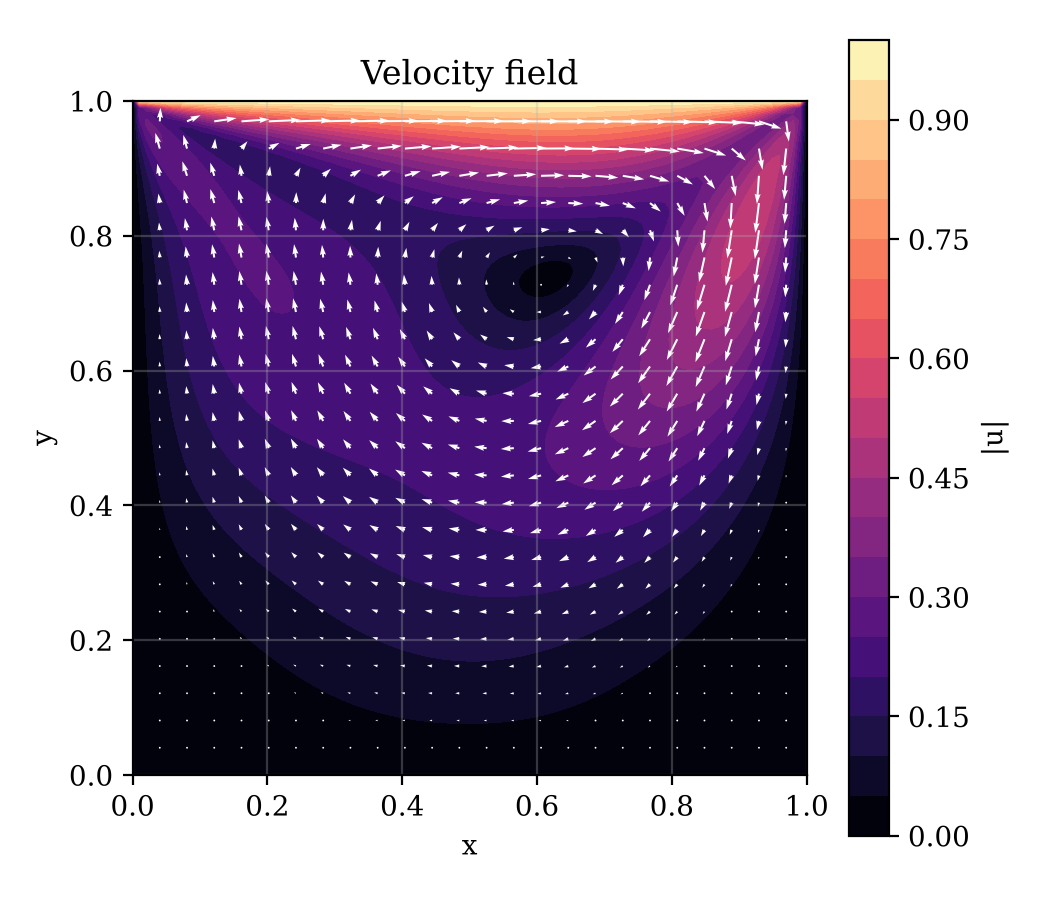
\includegraphics[width=0.55\textwidth]{../results/fig4_velocity_vectors.png}
\caption{Velocity vectors over speed contours.}\end{figure}
The flow consists of a primary clockwise vortex displaced towards the downstream (right) upper corner and two weak counter-rotating eddies in the bottom corners. The vorticity is concentrated in the lid boundary layer and is singular at the two lid corners, where the velocity jumps from 1 to 0; the downstream corner is a stagnation region of high pressure, and the pressure minimum coincides with the vortex core, where the radial pressure gradient balances the centripetal acceleration.

\subsection{Validation against Ghia et al.\ (1982)}
\begin{figure}[H]\centering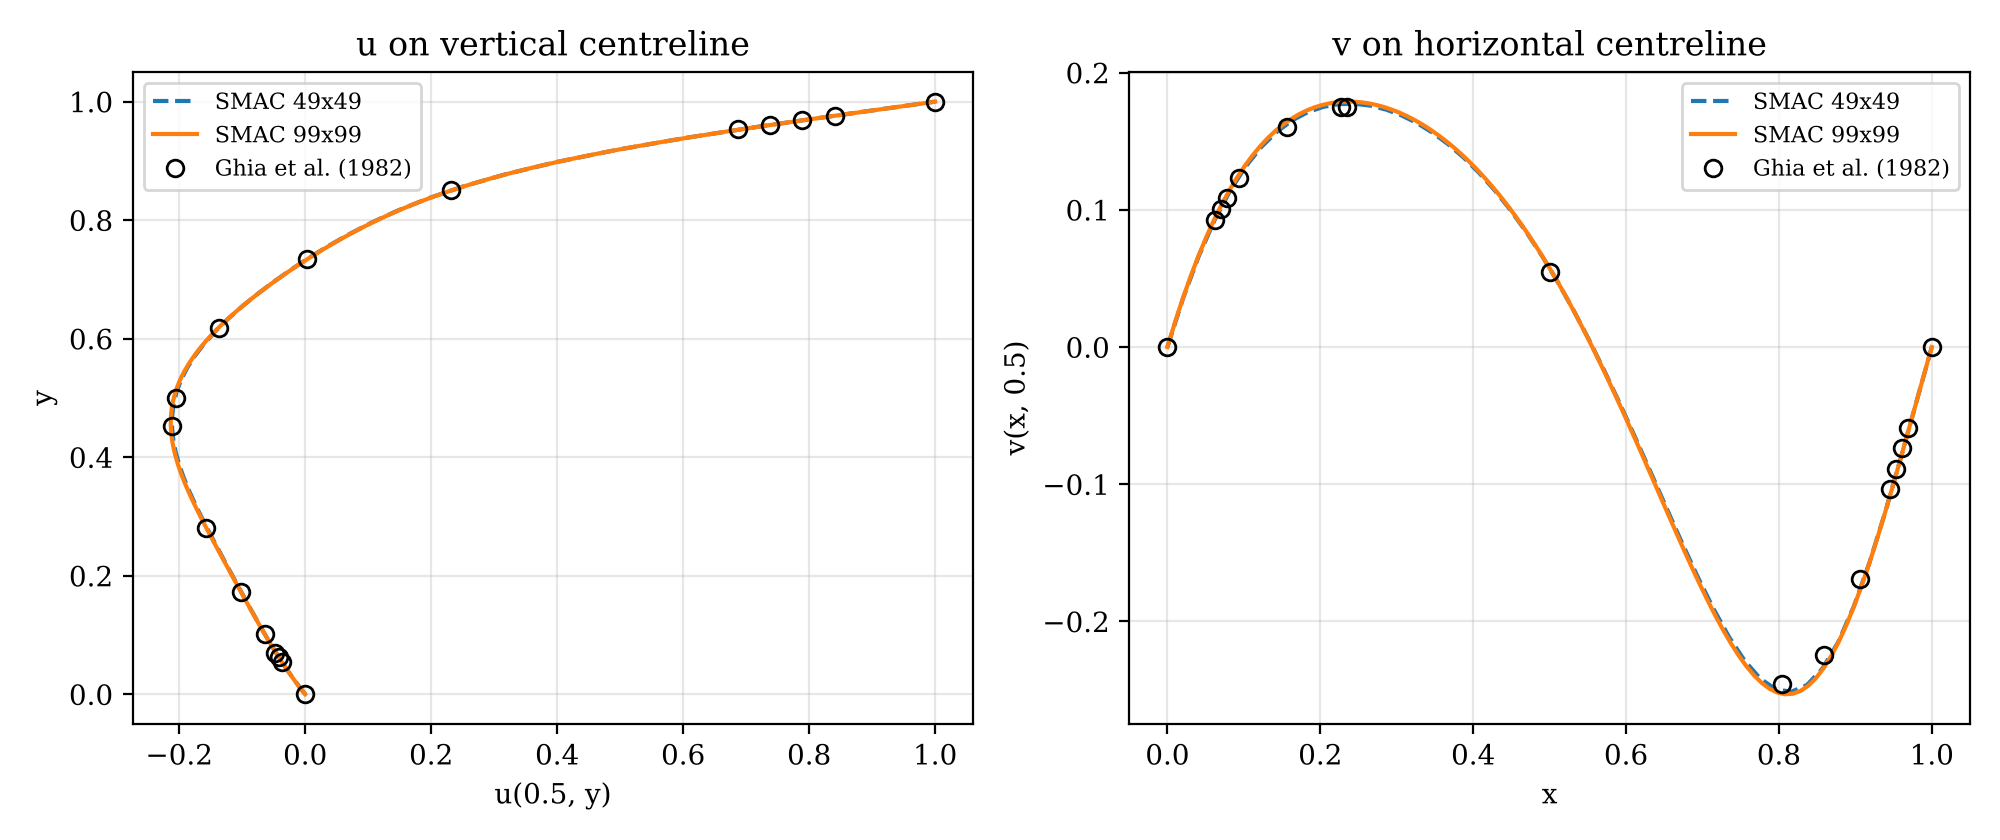
\includegraphics[width=\textwidth]{../results/fig2_centreline_vs_ghia.png}
\caption{Centreline velocity profiles against the benchmark of Ghia, Ghia \& Shin (1982), $129\times129$ multigrid stream function--vorticity solution.}\end{figure}
\begin{table}[H]\centering\small
\begin{tabular}{lccc}\toprule
Quantity & $49\times49$ & $99\times99$ & Ghia et al.\ (1982)\\\midrule
$\psi_{min}$ (primary vortex) & $-0.10294$ & $-0.10337$ & $-0.10342$\\
Primary centre $(x,y)$ & $(0.612,\,0.735)$ & $(0.616,\,0.737)$ & $(0.617,\,0.734)$\\
$\psi_{max}$ bottom-right eddy & $1.62\times10^{-5}$ & $1.35\times10^{-5}$ & $1.25\times10^{-5}$\\
$\psi_{max}$ bottom-left eddy & $3.24\times10^{-6}$ & $2.13\times10^{-6}$ & $1.75\times10^{-6}$\\
$u_{min}$ on $x=0.5$ & $-0.2112$ & $-0.2133$ & $-0.2109$\\
$v_{max}$ / $v_{min}$ on $y=0.5$ & $0.1773$ / $-0.2513$ & $0.1789$ / $-0.2531$ & $0.1753$ / $-0.2453$\\
$\max|u-u_{Ghia}|$ / rms & 0.0048 / 0.0020 & 0.0049 / 0.0022 & --\\
$\max|v-v_{Ghia}|$ / rms & 0.0077 / 0.0037 & 0.0088 / 0.0044 & --\\\bottomrule
\end{tabular}\caption{Comparison with the benchmark.}\end{table}
The primary vortex strength and position agree with the benchmark to $0.05\%$ and within one cell. The secondary eddies, which are four to five orders of magnitude weaker, converge monotonically towards the benchmark values under refinement. The centreline discrepancies ($\le0.009$, i.e.\ $<1\%$ of $U$) are of the same size as the uncertainty of the benchmark itself, which was computed on a $129\times129$ grid with a different formulation; later grid-converged studies report $u_{min}\approx-0.214$ at $\mathrm{Re}=100$ (e.g.\ Marchi et al., 2009), which the $99\times99$ value ($-0.2133$) approaches from the coarse-grid side.

\section{Conclusions}
\begin{itemize}
\item The completed SMAC solver on a staggered grid reproduces the classical Re $=100$ cavity solution: $\psi_{min}=-0.1034$ at $(0.616,0.737)$, both corner eddies, and centreline velocities within $<1\%$ of the lid speed of Ghia et al.
\item The staggered arrangement and the incremental pressure correction give a checkerboard-free pressure field and a Poisson cost that falls to $\sim10$ SOR sweeps per step near steady state.
\item The original code crashed (uninitialised variable-length arrays) and, even without the crash, contained no momentum equation, no continuity constraint and no lid boundary condition. Its structure was preserved and the numerical core completed; this is documented so the revised work can be presented accurately.
\end{itemize}

\section*{References}
\small
U.\ Ghia, K.N.\ Ghia, C.T.\ Shin, High-Re solutions for incompressible flow using the Navier--Stokes equations and a multigrid method, \emph{J.\ Comput.\ Phys.} 48 (1982) 387--411.\\
A.A.\ Amsden, F.H.\ Harlow, A simplified MAC technique for incompressible fluid flow calculations, \emph{J.\ Comput.\ Phys.} 6 (1970) 322--325.\\
F.H.\ Harlow, J.E.\ Welch, Numerical calculation of time-dependent viscous incompressible flow of fluid with free surface, \emph{Phys.\ Fluids} 8 (1965) 2182--2189.\\
C.H.\ Marchi, R.\ Suero, L.K.\ Araki, The lid-driven square cavity flow: numerical solution with a $1024\times1024$ grid, \emph{J.\ Braz.\ Soc.\ Mech.\ Sci.\ Eng.} 31 (2009) 186--198.
\normalsize
\section*{Reproducing the results}
\texttt{bash run.sh} builds and runs the $99\times99$ and $49\times49$ cases and calls \texttt{code/postprocess.py}.

\appendix\section{Source code}
\lstinputlisting[language=C]{../code/smac_cavity.c}
\end{document}
